\chapter{Building a data set for Comparative Argument Mining}
Due to the novelty of Argument Mining (and especially Comparative Argument Mining), the supply of datasets is small. Thus, a new data set had to be created.

This dataset was designed to answer the questions if a given sentence compares two known objects, and if it does, if the first-mentioned object is better or worse than the second one. Those questions will be translated to several classification tasks in the later chapters.

The dataset was created using the crowdsourcing platform CrowdFlower\footnote{https://www.crowdflower.com 23.02.2018}. As described in detail in the following chapters, the annotators were asked to assign one of four (and later three) classes to a sentence in which the objects of interest are highlighted.

The final dataset consists of 7421 sentences, each containing one of 273 object pairs. The sentences were labelled with one of three classes. Each sentence was at least annotated by three different annotators.

\section{Common Crawl Text Corpus}
The sentences for the crowdsourcing campaign were obtained from a CommonCrawl\footnote{https://commoncrawl.org 23.02.2018} dataset. CommonCrawl is a non-profit organisation which crawls the web and releases the crawled data for free use.

The data used in this thesis was already preprocessed\footnote{Download Link} (see \cite{Panchenko:2017aa}). First, it contains only English text. Duplicates and near-duplicates were removed, as well as all HTML tags. The texts were then split into sentences.

The resulting sentences were used to obtain the sentences for the crowdsourcing campaign. To make them manageable, an ElasticSearch index (from now on called "the index") was created. The index contains 3,288,963,864 unique sentences.

To get an idea if there are enough comparative sentences in the index, it was queried for all sentences containing one of the words \enquote{\emph{better}} or \enquote{\emph{worse}},  as those words often indicate a comparison. This query returns 32,946,247 matching sentences. Querying for \enquote{\emph{is better than}} still returns 428,932 sentences.

Those numbers show that there are enough sentences in the index to create a dataset for the given task. Even if only 1\% of the sentences containing \enquote{\emph{is better than}} are truly comparative, there would be 4289 training examples for the machine learning algorithm.


\section{Prestudies}
Before the mainstudy could start, several questions had to be answered.

First, how to extract sentences from the index? Second, how to preprocess those sentences? Third, which labels should be assigned to the sentences? Fourth, how to phrase the guidelines?

Two prestudies were conducted to answer those questions.



\subsection{Sentence Selection}
The sentences for the crowdsourcing campaign should have a high probability of being comparative so that enough positive examples for the machine learning part are present. To ensure this, a list of cue words which indicate comparison was compiled. For the prestudy, those words were \enquote{\emph{better}}, \enquote{\emph{worse}}, \enquote{\emph{inferior}}, \enquote{\emph{superior}}, and \enquote{\emph{because}}. Comparable objects are needed as well. A list of object pairs was selected by hand (see table \ref{tbl:prestudy-objects}). The pairs were selected in a way that they span a wide range of different domains, such as programming languages, countries and pets. The idea behind this is that pets are compared differently than programming languages. In this way, there will be different comparison patterns in the data.

\begin{table}[h]
\centering
\caption{Objects of the Annotation Prestudy}
\label{tbl:prestudy-objects}
\begin{tabular}{@{}llrrr@{}}
\toprule
First Object & Second Object      & \# Sentences                             \\ \midrule
Ruby    & Python    & 100      \\
BMW    & Mercedes    & 100  \\
USA & Europe & 100 \\
Beef & Chicken & 100   \\
Android & iPhone    &   100  \\
Cat & Dog      &     100  \\ 
Football & Baseball   &  100 \\ 
Wine & Beer  & 100  \\
Car & Bicycle & 100 \\
Summer & Winter &  100\\
\bottomrule  
                               
\end{tabular}
\end{table}

However, not all comparisons will contain one of the cue words mentioned above. Two different queries were used to overcome the coverage problem. Sevenhundred-fivtey sentences were obtained using query \ref{lst:es-query-a} (seventy-five for each pair) and 250 using query \ref{lst:es-query-b} (twenty-five for each pair). The second query will also match not-anticipated sentences such as \enquote{\emph{I like X more than Y since Z.}}.



\begin{lstlisting}[label=lst:es-query-a,breaklines=true,postbreak=\mbox{\textcolor{red}{$\hookrightarrow$}\space},caption=Prestudy Sentence Selection Query A]
{ "query":{  "bool":{ "must":[ {
          "query_string":{
            "default_field":"text",
            "query":"(better OR worse OR superior OR inferior) AND \"<OBJECT_A>\" AND \"<OBJECT_B>\""
          }
        } ] } } }
\end{lstlisting}

\begin{lstlisting}[label=lst:es-query-b,breaklines=true,postbreak=\mbox{\textcolor{red}{$\hookrightarrow$}\space},caption=Prestudy Sentence Selection Query B (shortened)]
[...]
          "query_string":{
            "default_field":"text",
            "query":" \"<OBJECT_A>\" AND \"<OBJECT_B>\""
[...]
\end{lstlisting}

Table \ref{tbl:example_sentences} shows some sentences obtained with this method. The objects of interest ar printed in italics.

\begin{table}[h]
\centering
\caption{Extracted Sentences}
\label{tbl:example_sentences}
\begin{tabular}{@{}llr@{}}
\toprule
 Sentence   &  Cue Words Used                      \\ \midrule
 He's the best pet that you can get, Better than a \emph{dog} or \emph{cat}. & Yes \\
\emph{Android} phones have better processing power than \emph{iPhone} & Yes \\
 10 Things \emph{Android} Does Better Than \emph{iPhone} OS & Yes \\
 \emph{Dog} scared of \emph{cat} & No \\
 In fact, many 'supercars' will use \emph{BMW} or \emph{Mercedes} engines. & No \\

\bottomrule  
                               
\end{tabular}
\end{table}



\subsection{Prestudy A}
The first prestudy had two goals. First, it should assess if the sentence selection method returns enough comparative sentences. Second, the design of the study as described below should be checked. On that account, a crowdsourcing campaign with one hundred of the 1000 sentences was started.



For each sentence, the annotators should decide to which class a sentence belongs. The classes are described in table \ref{tbl:prestudyclasses-a}. The classes \texttt{BETTER}, \texttt{WORSE} and \texttt{NO\_COMP} directly refer to the problem stated at the beginning of this chapter. The class \texttt{UNCLEAR} was added to capture all sentences which are somehow comparative but do not fit into the classes \texttt{BETTER} or \texttt{WORSE}.

\begin{figure}[h]
\centering
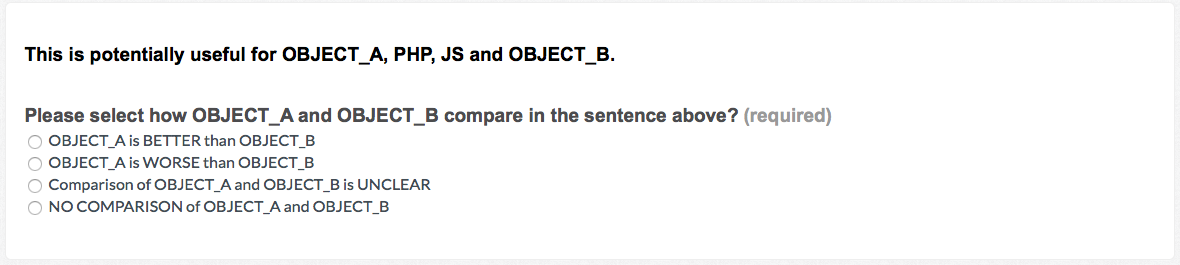
\includegraphics[width=1\textwidth]{images/prestudy/1_question}
\label{img:1_question}
\caption{Annotator view (Prestudy A)}
\end{figure}

\begin{table}[h]
\centering
\caption{Classes for Prestudy A and B}
\label{tbl:prestudyclasses-a}
\begin{tabular}{@{}ll@{}}
\toprule
Class & Description \\ \midrule
BETTER & The first object in the sentence (object A) is better than the second one (object B)\\
WORSE & The first object is worse \\
UNCLEAR & Neither BETTER nor WORSE fits, but the sentence is comparative\\
NO\_COMP & The sentence is not comparative or the sentence is a question\\
\bottomrule
\end{tabular}
\end{table}

In each sentence, the first object of interest was replaced with \texttt{OBJECT\_A}, while the second one was replaced with \texttt{OBJECT\_B}. Table \ref{tbl:pre_1_res} shows examples of processed sentences. The idea behind this was to enable the annotators to quickly see which objects should be taken into account for assigning a class. For example, in sentence three of table \ref{tbl:pre_1_res}, the annotator might be confused which of the objects are of interest, yet the replacement makes it clear that he should ignore \emph{C} and \emph{VB}. The view of the annotator (for a single sentence) is shown in figure \ref{img:1_question}.

Per batch, each annotator saw five sentences to annotate. He was also able to look into the annotation guidelines anytime he wanted. To filter out low-quality annotators, twelve sentences were selected as test questions. Each participant took a quiz (eight test questions) before the actual annotation process. One of the five sentences of the batch was a test question as well. If the annotator missed more than 30\% of the test questions, he was removed from the task. 

Figure \ref{fig:dist_pre_a} shows the resulting class distribution. The numbers after the class names show the absolute members of that class. As 45\% of the sentences are comparative, the selection procedure works satisfying.

\begin{figure}[h]
\centering
\caption{Class Distribution (Prestudy A)}
\label{fig:dist_pre_a}
\begin{tikzpicture}
\pie [rotate=180, text = legend, color= {cgray, cgreen, cred, cblue}]
    {55/NO\_COMP (55),
    15/BETTER (15),
    8/WORSE (8),
    22/UNCLEAR (22)}
\end{tikzpicture}
\end{figure}

The agreement of the annotators was acceptable. For thirty-seven sentences, all annotators agreed on one classes. Only for five sentences, each annotator assigned a different class. The remaining fifty-eight sentences got two different classes.

\begin{table}[h]
\centering
\caption{Uncertain Sentences (Prestudy A)}
\label{tbl:pre_1_res}
\begin{tabularx}{\textwidth}{lXrrr}
\toprule
\# & Sentence        & Ann. 1  & Ann. 2 & Ann. 3             \\ \midrule
1 & The only reason OBJECT\_A is used over OBJECT\_B, is because of libraries... & WORSE & UNCLEAR & NO\_COMP\\
2 & Agile development is the most popular model at the moment because of architectures like OBJECT\_A on Rails and Django (for OBJECT\_B) & NO\_COMP & NO\_COMP & UNCLEAR\\
3 & Your C# and VB devs can suddenly easily write web apps and your OBJECT\_A and OBJECT\_B devs can too - with the added bonus of much better performance &  NO\_COMP & NO\_COMP & UNCLEAR \\
4 & I'm a huge OBJECT\_A/Django \& OBJECT\_B/Rails fan, but I will never stop using PHP because it is so broadly accepted and supported & NO\_COMP & UNCLEAR & UNCLEAR \\
5 & It's why I mention OBJECT\_A and OBJECT\_B, because they've at least heard of them. & NO\_COMP & NO\_COMP & UNCLEAR \\


\bottomrule                              
\end{tabularx}
\end{table}

Some uncertain sentences are shown in table \ref{tbl:pre_1_res}, which displays the sentence and the decision of each annotator. As one can see in sentence two to five, annotators frequently were not able to distinguish between \texttt{NO\_COMP} and \texttt{UNCLEAR}. This is the case in fifty-one of the fifty-eight cases were two different classes were assigned.\newline

Fourteen out of fifty-five participants took part in an exit survey to rate the task. The overall satisfaction was rated with 3.2 out of 5. While the instructions (4.5), difficulty (4.4) and payment (3.8) got acceptable to good ratings, the test questions (2.9) were critizied. Also, 32 potential annotators failed the quiz. A second prestudy was conducted to adress the discovered problems.







\subsection{Prestudy B}
In the second prestudy, 200 sentences were annotated. Some changes in the task design were made to address the shortcomings of the first study.

Some points were identical to the first study. As the sentence selection process worked fine, the same 1000 base sentences were used in the second prestudy.  Each sentence was annotated by three annotators. They had to pass a quiz of eight test questions and had to keep an accuracy of 70\% on the test questions during the annotation procedure. The classes were the same as well.

The title of the task now contained the information that some computer knowledge is required for this task, as some pairs come from this domain. 
To address the problem with the confusion between \texttt{UNCLEAR} and \texttt{NO\_COMP}, the wording on this classes was changed. The new view of the annotator is displayed in figure \ref{img:2_question}. 
In the first prestudy, some annotators complained that the test questions were not fair. In fact, they contained some special cases so that they did not represent the whole dataset in an appropriate way. In the second prestudy, fifty-one test questions were used, who cover a wider range of examples.

The sentence preprocessing was altered as well. Instead of replacing the object, \mbox{\textbf{{\color[HTML]{9A14B2}:{[}OBJECT\_A{]}}}} or \textbf{{\color[HTML]{6CB219}:{[}OBJECT\_B{]}}} was appended. The colon and square brackets emphasize where the object of interest ends and the suffix begins. The idea behind this was, that the removal of the objects also removes some context from the sentences, which might be needed to classify them correctly. For further highlighting, the objects had a different colour.\newline

\begin{figure}[h]
\centering
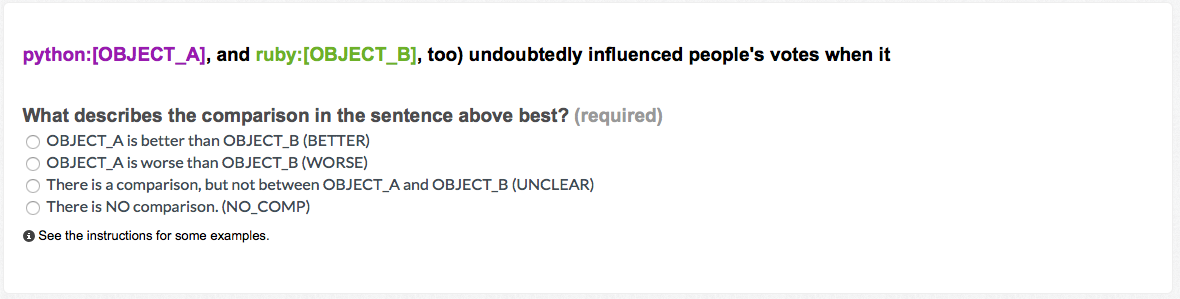
\includegraphics[width=1\textwidth]{images/prestudy/2_question}
\label{img:2_question}
\caption{Annotator view (Prestudy B)}
\end{figure}

The resulting class distribution is presentend in figure \ref{fig:dist_pre_b}. 

\begin{figure}[h]
\centering
\caption{Class Distribution (Prestudy B)}
\label{fig:dist_pre_b}
\begin{tikzpicture}
\pie [rotate=180, text = legend, color= {cgray, cgreen, cred, cblue}]
    {48/NO\_COMP (96),
    27/BETTER (54),
    11.5/WORSE (23),
    13.5/UNCLEAR (27)}
\end{tikzpicture}
\end{figure}

As in the first prestudy, nearly half of the sentences are somewhat comparative. For 125 (62.5\%) sentences, all annotators agreed on one class. Four (2.0\%) sentences got three different classes, for the remaining seventy-one (35.5\%) sentences two of the three annotators agreed on one class. The confusion between \texttt{UNCLEAR} and \texttt{NO\_COMP} is still the main problem for the sentences where only two annotators could agree. However, in the second prestudy this confusion only makes up fourty-five out of the seventy-two cases (62.5\% instead of 87.9\% in the first prestudy). Compared to the first prestudy, the amount of sentences where all annotators agreed on one class increased from 37\% to 62.5\%. 

\begin{table}[h]
\centering
\caption{Uncertain Sentences (Prestudy B)}
\label{tbl:pre_1_res}
\begin{tabularx}{\textwidth}{lXrrr}
\toprule
\# & Sentence        & Ann. 1  & Ann. 2 & Ann. 3             \\ \midrule
6 & Google shouldn't have mandated an inferior map app on the iphone:[OBJECT\_A] (as opposed to android:[OBJECT\_B]). & BETTER & WORSE & NO\_COMP \\
7 & (See android:[OBJECT\_A] Dethrones the iphone:[OBJECT\_B] .) & BETTER & NO\_COMP & NO\_COMP \\
8 & android:[OBJECT\_A] didn't out pace the iphone:[OBJECT\_B] this year, it just sold slightly better in America & WORSE & NO\_COMP & WORSE\\
9 & To me it is much better than iphone:[OBJECT\_A] and android:[OBJECT\_B]. & NO\_COMP & UNCLEAR & UNCLEAR \\
10 & ( android:[OBJECT\_A] , Crush , iPad , iphone:[OBJECT\_B] )& NO\_COMP & BETTER & NO\_COMP \\

\bottomrule                              
\end{tabularx}
\end{table}


From 125 candidate annotators, thirty-five failed the initial quiz. Twelve annotators were removed during the annotation process as they answered too many test questions wrong.
Twenty-two annotators took the exit survey. The overall satisfaction increased to 3.7 out of 5. The test question fairness was now rated with 3.7 out of 5 instead of 2.9. The rating for the payment slightly increased to 3.9, yet the payment was not changed. However, the rating for the instructions decreased to 3.9 and for the difficulty to 3.5.
The change in numbers is explained by the increased amount of sentences, which introduce new cases which are not directly reflected in the annotation guidelines. However, as only a small fraction of the annotators took the exit survey in both prestudies, the results can only be used as one signal. The annotation results are another, more important signal, and they are convincing.

\subsection{Validation of results}

Due to an error in the creation of the crowdsourcing task, the sentences where not shuffled. This means that the first one-hundred sentences of the second prestudy are the same as the one-hundred sentences of the first prestudy. Another problem is the bias: except for X sentences, all other sentences contained the pairs X and Y. However, since the goal of the prestudy was mainly to assess the sentence selection method and the guidelines, this does not invalidate the results. This problems were removed in the main study.
%\subsection{Task}
%
%\textbf{ALT ALT ALT ALT ALT}
%Using the method described above, 1050 sentences were obtained for the prestudy. The annotators were asked to assigne one of the following classes to the sentences. Each sentence was annotated by three annotators.
%
%The annotators where asked to assign one of the four classes (see table \ref{tbl:prestudyclasses}) to each sentence.
%
%
%
%
%
%In a first step, 100 sentences were annotated. To ensure the quality, twelve additional sentences were setup as test sentences. If one annotator failed three test sentences, he was removed from the task.
%
%The sentences were preprocessed: the first object was replaced by OBJECT\_A, the second by OBJECT\_B. Examples are shown in table \ref{tbl:pre1s}. The removal was done so that the annotators can concentrate on the comparative structure of the sentence and are not biased by the objects.
%
%
%% Beispielsätze PreStudy 1. Teil
%
%
%
%This test step delivered valuable insights. First, the amount of test sentences was to small. Users might see the same test sentence twice. Second, the phrasing of the annotation guidelines was to confusing, especially the distinction between NO\_COMP and UNCLEAR as well as their class names.
%Third, the complete removal of the original objects is suspected to partly obscure the sense of the sentences.\newline
%
%In a second step, 200 new sentences were annotated, again with three annotations per sentences. This time, 51 test questions were used, so that it is less likely that annotators will see the same question twice. Furthermore, the preprocessing was changed. Instead of removing the original objects, :[OBJECT\_A] was appended to the first object, :[OBJECT\_B] to the second object. Also, each object was highlighted in a different color. Example sentences are shown in table \ref{tbl:pre2s}. In this way, the annotators could quickly see the objects of interest while the sense of the sentence remains intact.
%% Beispielsätze PreStudy 2. Teil
%\begin{table}[h]
%\centering
%\caption{Sentences for the second step}
%\label{tbl:pre2s}
%\begin{tabular}{{p{12cm}p{3cm}}}
%\toprule
%Sentence                                                                                                           & Expected Class \\ \midrule
%I'd go with \textbf{{\color[HTML]{9A14B2} python:{[}OBJECT\_A{]}}} or \textbf{{\color[HTML]{6CB219}ruby:{[}OBJECT\_B{]}}}.                                 & NO\_COMP       \\
%I prefer \textbf{{\color[HTML]{9A14B2}ruby:{[}OBJECT\_A{]}}} over \textbf{{\color[HTML]{6CB219}python:{[}OBJECT\_B{]}}} on windows.                                              & BETTER         \\
%I've tried \textbf{{\color[HTML]{9A14B2}python:{[}OBJECT\_A{]}}}, and can see why people like it, but \textbf{{\color[HTML]{6CB219}ruby:{[}OBJECT\_B{]}}} suits my style better. & WORSE          \\
%i think this car is a far better deal than the \textbf{{\color[HTML]{9A14B2}bmw{:[OBJECT\_A]}}} 5 series or \textbf{{\color[HTML]{6CB219}mercedes:[OBJECT\_B]}} 320e.                                                                                                                &        UNCLEAR        \\ \bottomrule
%\end{tabular}
%\end{table}
%
%\label{sec:annotation-guidelines}
%\subsection{Results}
%Each sentence was annotated by three annotators. Figure \ref{pre:dist} shows the class distribution.
%
%\begin{figure}[h]
%\centering
%\caption{Class Distribution in the prestudy}
%\label{pre:dist}
%\begin{tikzpicture}
%\pie [rotate=180, text = legend, color= {cgray, cgreen, cred, cblue}]
%    {59.76/NO\_COMP (150),
%    23.11/BETTER (58),
%    9.16/WORSE (23),
%    7.97/UNCLEAR (20)}
%\end{tikzpicture}
%\end{figure}
%
%
%%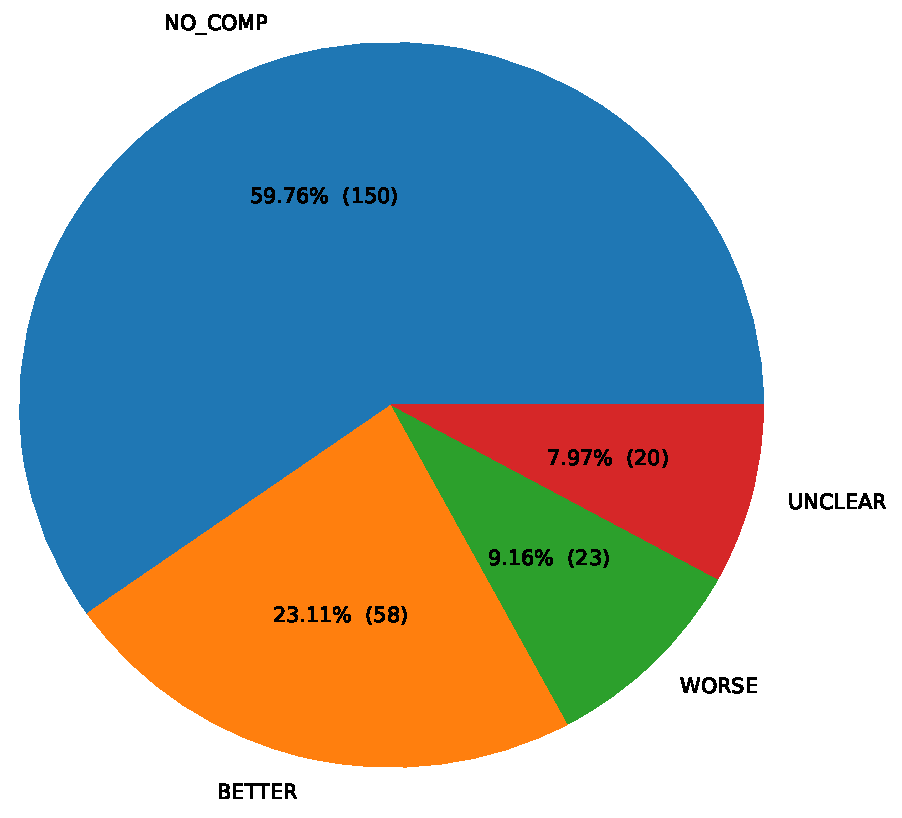
\includegraphics[scale=0.6]{images/prestudy/label_distribution.pdf}
%
%
%Crowdflower has a trust value for each annotator. This trust value and the number of votes per class gives a value of confidence for each label.\footnote{How the confidence is calculated in detail can be found at https://success.crowdflower.com/hc/en-us/articles/201855939-How-to-Calculate-a-Confidence-Score (Last checked: 19.12.2017)}
%
%
%As presented in figure \ref{pre:conf}, a majority (151) of the labelings has a confidence greater or equal to 0.9, and 15 sentences a confidence below 0.6; the mean is 0.86. Detailed numbers on the confidence are shown in table \ref{pre:conf-table}
%
%\begin{figure}
%\centering
%\caption{Confidence histogram}
%\label{pre:conf}
%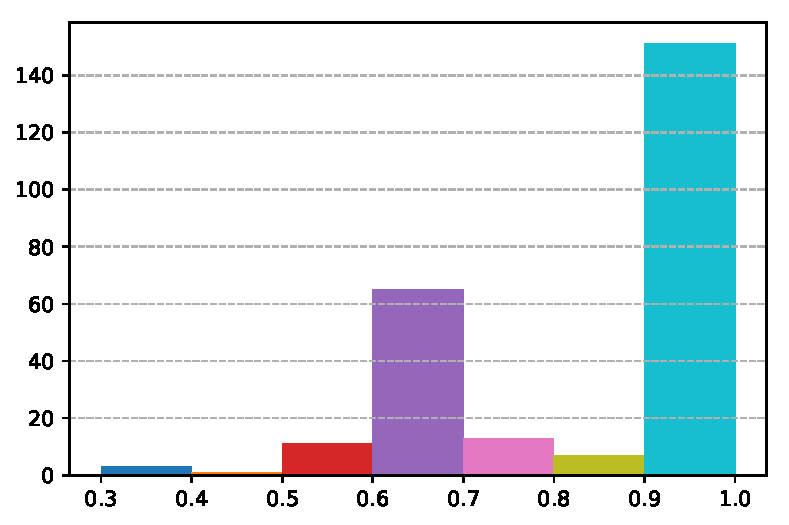
\includegraphics[scale=0.6]{images/prestudy/confidence.pdf}
%\end{figure}
%
%
%\begin{figure}[h]
%\centering
%\caption{Confidence}
%\begin{tabular}{@{}ll@{}}
%\toprule
%Type & Value  \\ \midrule
%Average Confidence & 0.86 \\
%Standard Derivation & 0.17 \\
%Lowest Confidence & 0.35\\
%Highest Confidence & 1.00\\
%25th percentile average & 0.67\\
%50th percentile average & 1.00\\
%\bottomrule
%\label{pre:conf-table}
%\end{tabular}
%\end{figure}
%
%
%
%
%
%The most difficult sentence is with a confidence of 0.35 for the class \emph{WORSE} was
%\begin{quote}
%Google shouldn't have mandated an inferior map app on the iphone:[OBJECT\_A] (as opposed to android:[OBJECT\_B]).
%\end{quote}
%
%It was labelled as \emph{BETTER} (trust: 0.72), \emph{WORSE} (trust: 0.85) and \emph{NO\_COMP} (trust: 0.82). The class \emph{WRONG} is correct here, as the object \enquote{iphone} is inferior to \enquote{android} on the aspect of \enquote{map app}.
%
%The following sentence was assigned to \emph{BETTER} (0.37 confidence), although it should belong to \emph{UNCLEAR}.
%\begin{quote}
%Not to mention that the iphone:[OBJECT\_A] and android:[OBJECT\_B] phones deliver a far superior user experience overall
%\end{quote}
%However, the annotator for \emph{UNCLEAR} only had 0.87 trust, while the one for \emph{BETTER} had 1 (third one was \emph{NO\_COMP} with 0.82 trust).\newline
%
%All things considered, the result of the prestudy is satisfactory. The annotators agreed in the majority of decisions. 


\newpage
\section{Main Study}
\label{sec:mainstudy}
\subsection{Task Description}
\subsection{Data Generation}
Three domains were fixed for the sentences of the main study. The domains were chosen in a way that a majority of people can decide whether a sentence contains a comparison or not.

The most specific domain was "Computer Science Concepts". It contains objects like programming languages, database products and technology standards such as Bluetooth and Ethernet.  Many computer science concepts can be compared objectively, for instance, one can compare Bluetooth and Ethernet on their transmission speed. Some basic knowledge of computer science was needed to label sentences correctly. For example, to compare Eclipse and NetBeans, the annotator must know what an Integrated Development Environment (IDE) is and that both objects are Java IDEs.  The need of the knowledge was communicated to the prospective annotators. The objects for this domain were manually extracted from "List of ..." articles from Wikipedia.

The second, broader domain was "Brands". It contains objects from of different types (car brands, electronics brands, and food). As brands are present in everyday life of people, it is expected that anyone can label the majority of sentences containing well known brands such as Coca-Cola or Mercedes. As with computer science, the objects for this domain were extracted from "List of ..." articles from Wikipedia.

The last domain is not restricted to any topic. For each one of 25 randomly selected seed words, ten similar words were extracted using JoBimText, a software package for distributional semantics. The seed words were created using https://randomlists.com\footnote{Last checked: 25.01.2018}. Listing \ref{lst:jbtres} shows the result\footnote{http://ltmaggie.informatik.uni-hamburg.de/jobimviz/ws/api/stanford/jo/similar/harvard\%23NP?numberOfEntries=10&format=json Last checked: 25.01.2018; Some uninteresting fields were removed for brevity} for the seed word \emph{harvard}.

\begin{lstlisting}[language=json,label=lst:jbtres,caption=Similar words to "Harvard"]
{
   "results":[
      { "score":688.0, "key":"harvard#NP" },
      { "score":245.0, "key":"yale#NP" },
      { "score":163.0, "key":"princeton#NP" },
      { "score":152.0, "key":"mit#NP" },
      { "score":143.0, "key":"stanford#NP" },
      { "score":133.0, "key":"university#NP"},
      { "score":132.0, "key":"tufts#NP" },
      { "score":130.0,"key":"cornell#NP"},
      { "score":127.0, "key":"nyu#NP" },
      { "score":113.0, "key":"university#NN" }
   ]
}
\end{lstlisting}
This method covers a wide are of possible comparison patterns.\newline

Especially for brands and computer science, the object lists are long (4493 brands and 1339 for computer science).The frequency of each object was checked using a frequency dictionary to reduce the number of possible pairs. All objects with a frequency of zero and ambiguous objects were removed from the list. For instance, the objects "RAID" (a hardware concept) and "Unity" (a game engine) were removed from the computer science list as they are also regularly used nouns.

The remaining objects were combined to pairs. For each type, all possible combinations were created. For brands and computer science, the type is the source list. For the unrestricted domain, the seed word was used. This procedure guarantees that only meaningful pairs are created.
The ElasticSearch Index was then queried for entries containing both objects of each pair. For 90\% of the queries, the marker terms where added to the query. This was done to check whether there is a chance that those two objects were compared. All pairs were the query yielded at least 100 sentences were kept. Those pairs are frequent enough and have a high chance of generating comparative sentences.

From the sentences of those pairs, 2500 for each category were randomly sampled as candidates for the crowdsourcing campaign. 250 sentences were manually labelled to check if there are enough comparative sentences. Those labels were discarded for the crowdsourcing campaign.
The label distribution of the 250 sentences is presented in the figures FIGURE NUMBERS.

\begin{figure}[h]
    \centering
    \begin{minipage}{0.49\textwidth}
        \centering
       \begin{tikzpicture}
\pie [rotate=180,radius=2,color= {cgray, cgreen, cred, cblue}]
    {68.9/NONE,
    15.2/BETTER,
    5.7/WORSE,
    10.2/OTHER }
    \label{pre:brands}
\end{tikzpicture}        \caption{Brands}
    \end{minipage}\hfill
    \begin{minipage}{0.49\textwidth}
        \centering
      \begin{tikzpicture}
\pie [rotate=180,radius=2, color= {cgray, cgreen, cred, cblue}]
    {53.00/NONE,
    19.70/BETTER,
    11.60/WORSE,
    15.70/OTHER }
\end{tikzpicture}
        \caption{Computer Science}
    \end{minipage}
    \end{figure}
    
    \begin{figure}[h]
    \centering
    \begin{minipage}{0.49\textwidth}
        \centering
       \begin{tikzpicture}
\pie [rotate=180,radius=2,color= {cgray, cgreen, cred, cblue}]
    {65.50/NONE,
    16.10/BETTER,
    7.20/WORSE,
    11.20/OTHER }
\end{tikzpicture}        \caption{Unrestricted}
    \end{minipage}\hfill
    \end{figure}
    
In all samples, at least 30\% of the sentences are comparative. This number shows that the sampling method is sufficient to sample sentences for the crowdsourcing campaign.
